\subsection{Documentación del código}

Debido a la alta modularidad del código y como se ha explicado previamente, ha sido dividido en módulos. Para simplificar la integración y legibilidad de dichos módulos, se han comentado extensivamente y se utiliza \texttt{Doxygen} para generar la página de la documentación en formato \texttt{HTML}.

Para ello, se deben utilizar comentarios con un formato muy marcado como el que se ve en el siguiente fragmento:

\begin{lstlisting}[caption={Ejemplo de comentario \texttt{Doxygen}},captionpos=b]
    /**
    * @brief Escribe la medida en el fichero indicado.
    * Formato: [timestamp] VPanelSolar: X.XX V, IPanelSolar: X.XX mA, VBatBackup: X.XX V, IBatBackup: X.XX mA, VBat1: X.XX V, IBat1: X.XX mA, VBat2: X.XX V, IBat2: X.XX mA
    * 
    * @param measFile Nombre del fichero.
    * @param measures Medidas a escribir.
    * @param timestamp Marca de tiempo.
    * @return true si la escritura fue exitosa, false en caso contrario.
    */
    extern bool write_meas(const char* measFile , telemetry_t measures, String timestamp);
\end{lstlisting}

Gracias a este formato estándar, se puede extraer toda la documentación y generar una web ({\url{https://david-andrino.github.io/iot-power}}) como la que se ve en la siguiente figura.

\begin{figure}[H]
    \centering
    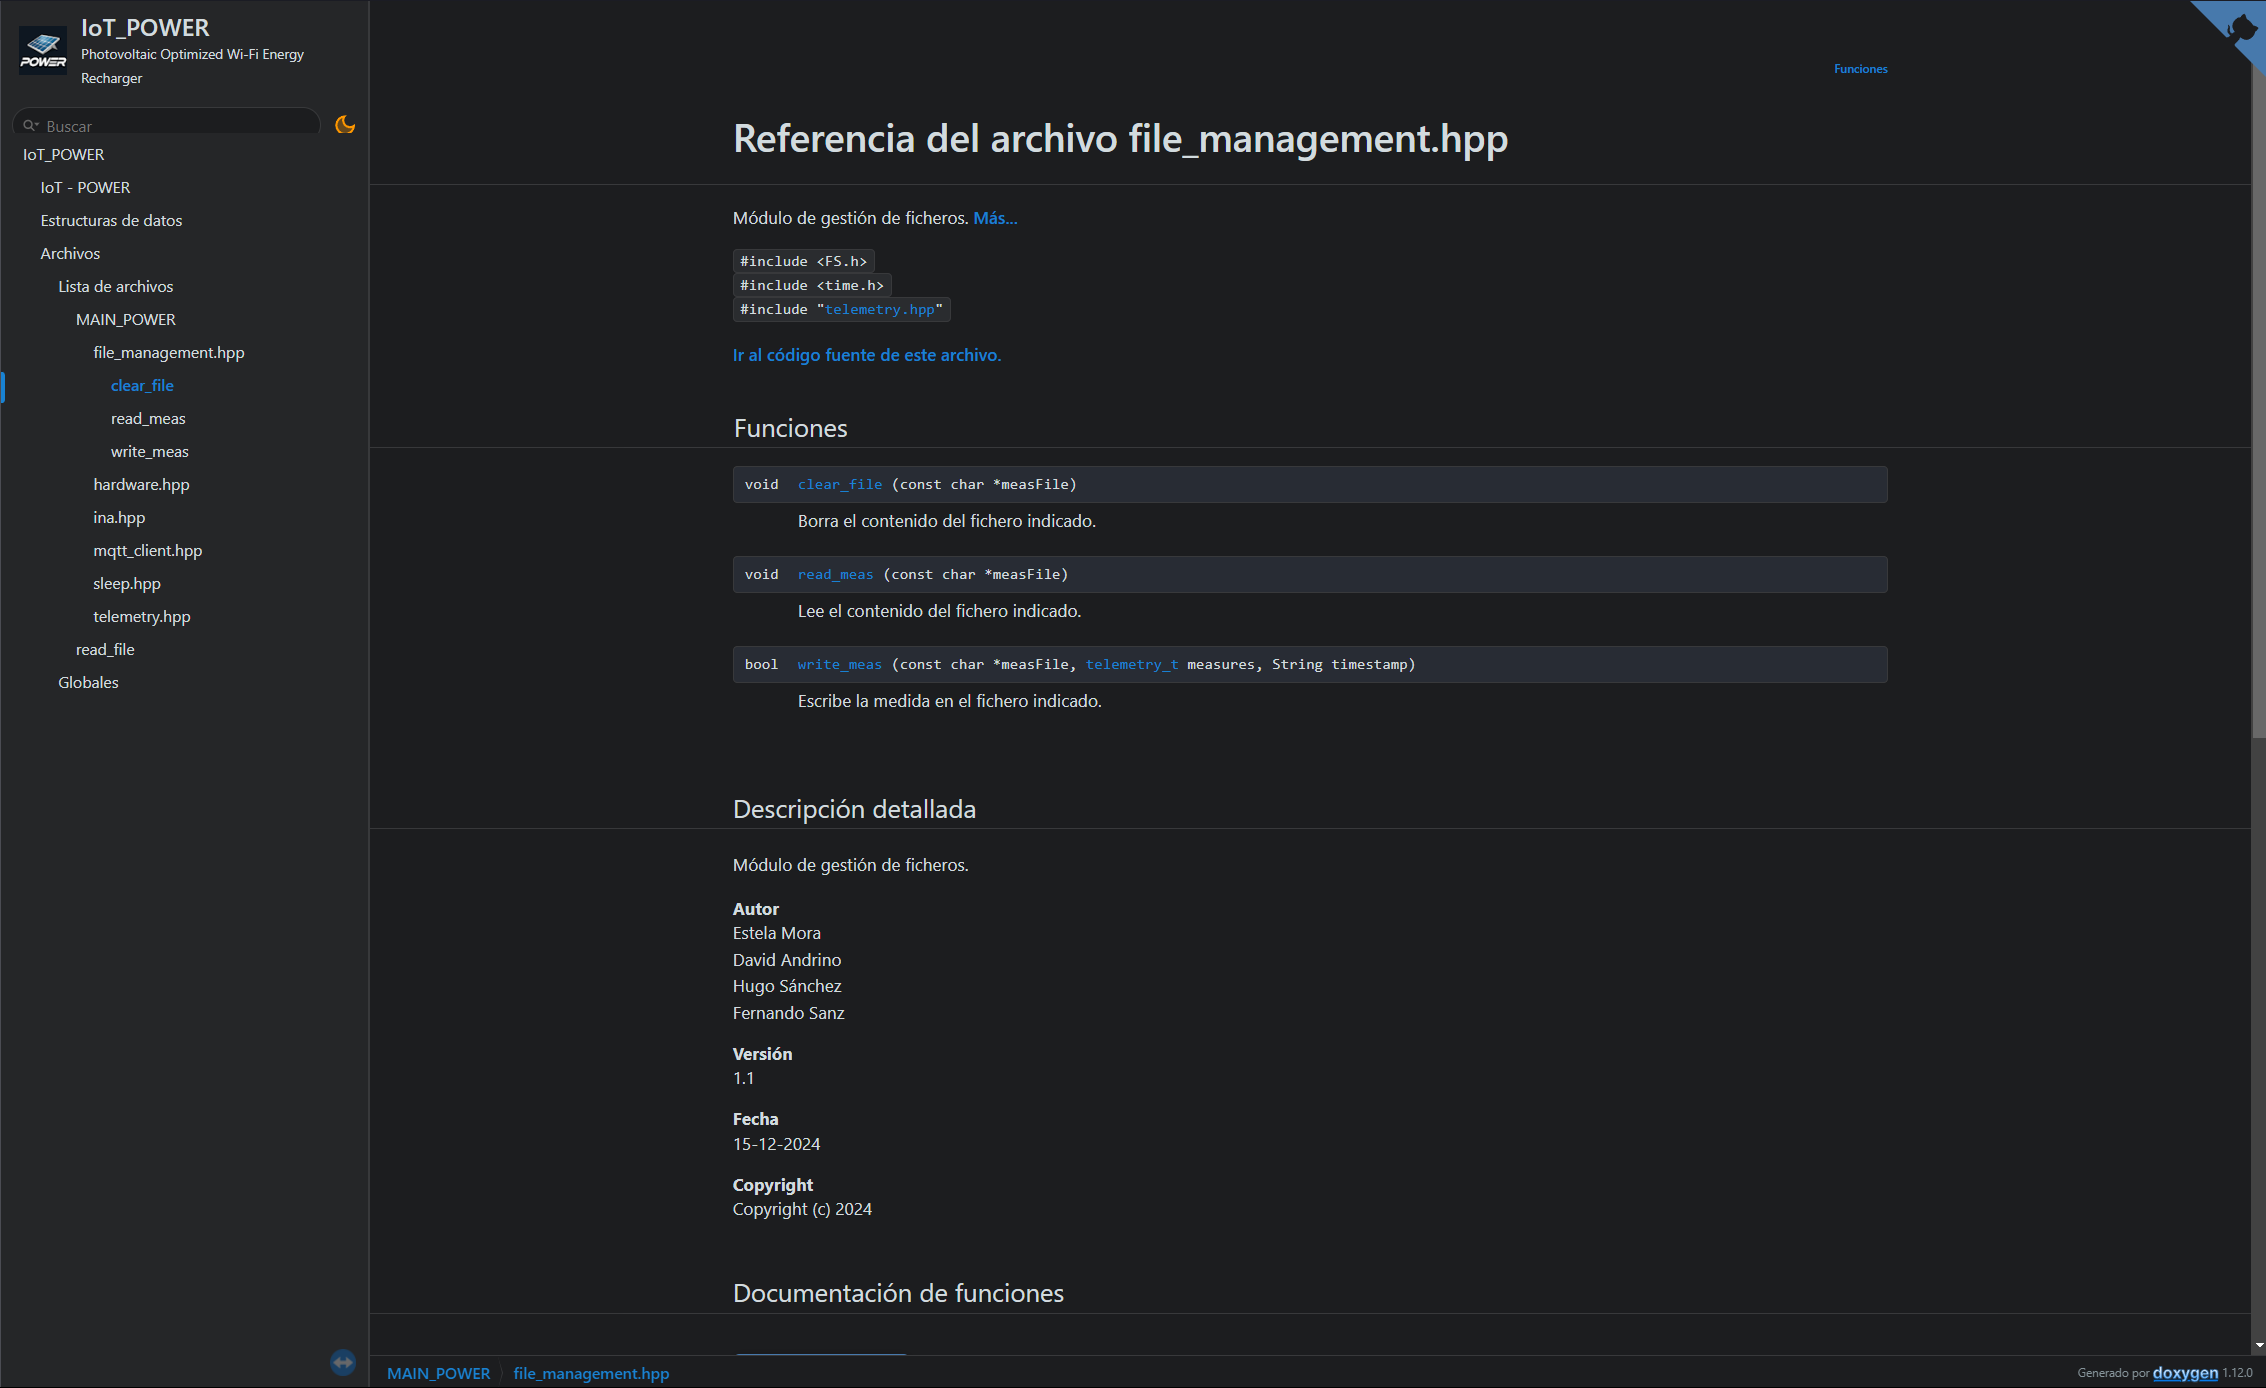
\includegraphics[width=0.8\textwidth]{images/3-software/3-5-doxygen/web.png}
    \caption{Captura de la web de documentación}
\end{figure}

Para automatizar la generación, se ha utilizado una \texttt{GitHub Action}, la cual genera automáticamente la documentación y la publica gracias a \texttt{GitHub Pages}. Esta acción y el tema de la documentación se han obtenido del repositorio \texttt{doxygen-awesome-css}. \cite{jotheproJotheproDoxygenawesomecss2024} 

Estas herramientas de \texttt{CI/CD} permiten agilizar altamente el desarrollo de dicha documentación, ya que esta se regenera y publica automáticamente después de cada \texttt{Commit} de la rama principal.

\begin{figure}[H]
    \centering
    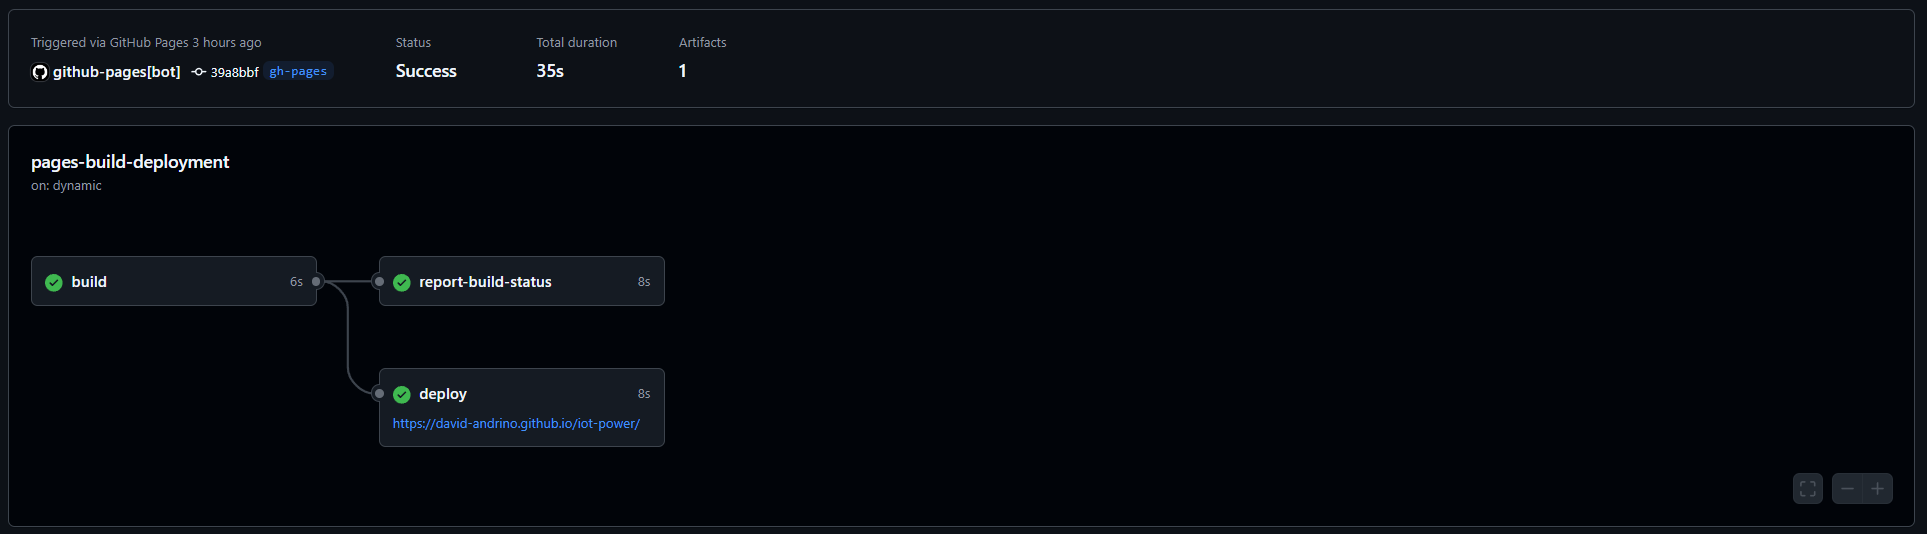
\includegraphics[width=0.9\textwidth]{images/3-software/3-5-doxygen/githubAction.png}
    \caption{\texttt{GitHub Action} para la generación de documentación}
\end{figure}